\documentclass[a4paper]{article}
\usepackage[hmargin=1in, vmargin=1in]{geometry}
\usepackage{makeidx}
\usepackage{fancyhdr}
\pagestyle{fancy}
\usepackage[pdftex]{graphicx}
\usepackage{amsmath}
\usepackage{amssymb}
\usepackage{listings}
\usepackage{natbib}
%\makeindex
\begin{document}
\begin{center}
\title{Transformation dreidimensionaler Koordinaten in zweidimensionale Koordinaten (German Version)}\\
\author{Edward Gerhold}
Transformation dreidimensionaler Koordinaten in zweidimensionale Koordinaten (German version)\\
\date{\today}
\maketitle


Deutsche Version 0.0.98 von 0.1.0\\

\end{center} 

\tableofcontents\\

\section{Einleitung}

Auf einem Blatt Papier sehen wir ein dreidimensionales Koordinatensystem in den Raum zeigen.
In der Realit\"at sind die drei Basisvektoren der Abbildung zweidimensional. Denn sie zeigen 
in drei Richtungen, flach auf dem Papier, und gar nicht in den reellen Raum.\\

\begin{figure}[ht]
\label{ijksystem}
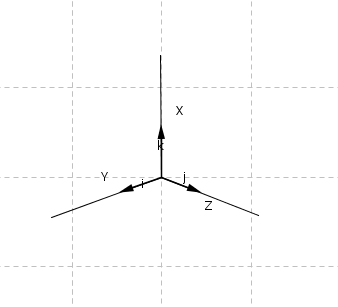
\includegraphics[scale=2]{ijksystem.png}\\
\caption{Bild eines rechtsh\"andigen Koordinatensystems mit ijk-Basisvektoren auf den Achsen, in drei dimensionen zeigend. Schauen sie in \cite{Corral1} f\"ur eine Einf\"uhrung.}
\end{figure}

In diesem Dokument entwerfen wir ein $\mathbb{R}^{2\times{3}}$ Koordinatensystem um 3-D Punkte in 2-D Punkte umzuwandeln.
Mit den Kosinus- und Sinusfunktionen errechnen wir die exakten Anteile der horizontalen und vertikalen Teilverschiebungen.\\

\textbf{Was wir in diesem Dokument machen werden.}

\begin{enumerate}
\item Winkel ausw\"ahlen f\"ur unsere Koordinatenachsen 
\item Einheiten der Achsen ausw\"ahlen oder sich f\"ur $1$ entscheiden
\item Die drei zweidimensionalen Achsvektoren des Koordinatensystems aufschreiben
\item Die Achsen zu einer Matrix, einer Funktion, oder anstelle der Basis zusammenbauen
\item Den JavaScript Code der Transformation lesen
\item In den Folgeversionen die noch nicht eingetragenen bereits bekannten Fakten kennenlernen

\end{enumerate}

%\chapter{1}

\section{Entwurf eines $\mathbb{R}^{2\times{3}}$ Koordinatensystems f\"ur unsere Koordinatentransformation vom $\mathbb{R}^{3}$ auf den $\mathbb{R}^{2}$}

In der englischen Version schreibe ich alles etwas anders. Diese deutsche Fassung ist speziell neu angefangen und ich verfolge das
Ziel, mich auch etwas k\"urzer zu fassen. Mathematik, die ich in der deutschen Fassung auslassen werde, ist aber problemlos in der
englischen Version zu verfolgen. Wer das rechnen kann, kann bestimmt auch ein wenig Englisch und versteht auch deutsches Englisch.\\

\subsection{Koordinatensystem}
\subsubsection{Links- und rechts}

Ein linksh\"andiges Koordinatensystem auf der Ebene hat die dritte Achse zwischen den beiden normalen Achsen in die gleiche Richtung zeigend.\\

\begin{figure}
\caption{Ein linksh\"andiges Koordinatensystem}
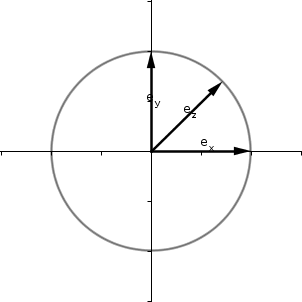
\includegraphics[scale=0.5]{lefthand45.png}
\end{figure}

Bei einem rechtsh\"andigen Koordinatensystem auf der Ebene zeigt die dritte Achse in die entgegengesetzte Richtung.\\

\begin{figure}
\caption{Ein rechtsh\"andiges Koordinatensystem}
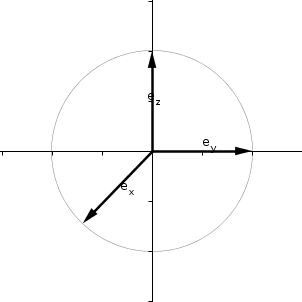
\includegraphics[scale=0.5]{righthand45.png}
\end{figure}

\subsubsection{Einheitskreis}

Der Einfachheit halber kann man die drei Achsen am Einheitskreis ausrichten. Dazu bedienen wir uns gleich einer hilfreichen Formel aus dem Polarkoordinatensystem.\\

\begin{displaymath}
	(x,y) := (r \cos \varphi, r \sin \varphi)
\end{displaymath}

$(x,y)$ stellen die Spitze eines Ortsvektors aus dem Ursprung des Koordinatensystems dar. Wenn wir drei Achsen haben wollen, sollten wir uns drei solche Vektoren, die von $(0,0)$ bis $(x=r_n\cos\varphi_n,y=r_n\sin\varphi_n)$ zeigen, deren L\"angen fuer die Einheit $1$ der jeweiligen Achse stehen, erzeugen. Das werden wir auch gleich tun. \\


\subsection{Winkel der Achsen}

Die Achsen werden von der horizontalen x-Achse des zweidimensionalen Bilds gegen den Uhrzeigersinn gez\"ahlt. Da wir drei Achsen haben, brauchen wir auch drei Winkel.\\

\begin{displaymath}
	\varphi_n := \{ \varphi_x, \varphi_y, \varphi_z | \mbox{ die Winkel der drei Achsen}\}
\end{displaymath}

Die Winkel kann man selbst in Grad oder Radians festlegen. Die Programmiersprache JavaScript zum Beispiel nimmt, f\"ur die Funktionen Kosinus und Sinus die Winkel, in Radians an. Die sind mit einer einfachen Formel berechenbar.\\

\begin{displaymath}
	\mbox{rad}(\mbox{deg}) := \frac{\pi}{180} \times \mbox{deg}
\end{displaymath}

\begin{displaymath}
	\mbox{deg}(\mbox{rad}) := \frac{180}{\pi} \times \mbox{rad}
\end{displaymath}

\subsection{Einheit der Achsen}

\subsubsection{Der r-Wert der Achsen}

Der r-Wert, den man als Radius in den Polarkoordinaten kennt, steht f\"ur die L\"ange des Ortsvektors. Er steht somit auch f\"ur die L\"ange unserer Achsen. Im angewandten Sinne kann man damit unseren drei Achsen die Abstand der Einheiten eingestellt werden.\\


\begin{displaymath}
	r_n := \{ r_x , r_y , r_z | \mbox{ die Einheit jeder der drei Achsen}\}
\end{displaymath}

Mit dem r-Wert $r_x = r_y = r_z = 1$ erhalten wir normalisierte Einheitsvektoren. In dem Fall kann $r_n$ ganz weggelassen werden.\\

Von der Norm der Achsvektoren handelt der Abschnitt \ref{Norm_Achsvektoren}


\subsubsection{Mathematische Vorsicht mit dem r-Wert}

\begin{enumerate}

\item Der r-Wert verkompliziert die Berechnungen und Absch\"atzungen nat\"urlich, weil die Koordinaten mit multipliziert werden. \\

\item Wenn man bewegte Bilder produzieren will, sollte der r-Wert grundsaetzlich gleich auf allen Achsen sein, weil Rotationen und Translationen sonst daneben gehen, da die Punkte dann pl\"otzlich ihre Einheiten wechseln. Das sieht bewegt unrealistisch aus, ist aber
bei Standbildern kein Problem. Es ist m\"oglich selbige Ver\"anderung lokal an den Objekten vorzunehmen, damit bleibt die Vergr\"osserung transformationsinvariant bez\"uglich den Drehungen.\\

\item Die Formel verkompliziert sich bei drei verschiedenen r-Werten nat\"urlich und zum Rechnen sollte zuerst das vereinfachte Modell
herangezogen werden, wo der r-Wert auf allen drei Achsen gleich ist, oder gleich $1$ ist und komplett entf\"allt.\\

\end{enumerate}

\subsection{(Basis)vektoren der Linearkombination}

Wir ben\"otigen f\"ur das Koordinatensystem drei Achsen. Jede Achse bekommt einen kanonischen Einheitsvektor $\begin{pmatrix}\cos\varphi_n\\\sin\varphi_n\end{pmatrix}$, wie er aus Unterricht und B\"uchern auch Nichtmathematikern bekannt ist. Allerdings behalte ich mir vor, das Koordinatensystem flexibel zu definieren, warum jeder Achsvektor mit dem r-Wert konfigurierbar ist.\\

\begin{displaymath}
\vec{e}_n := \{ \vec{e}_x, \vec{e}_y, \vec{e}_z | \vec{e}_n = \begin{pmatrix}r_n \cos \varphi_n\\r_n \sin \varphi_n\end{pmatrix}, \mbox{ die drei Achsen des Koordinatensystems }\}
\end{displaymath}

Wenn der r-Wert gleich $1$ ist, haben diese Vektoren gleich normalisierte Einheitsl\"ange im Sinne der Orthonormalbasis. Der Unterschied zur Orthonormalbasis ist, dass wir mindestens eine linear abh\"angige Achse haben. Je nach Arrangement um den Kreis k\"onnen dabei bis zu drei linear abh\"angige Achsen entstehen, in Bezug zur 2-D Standardbasis $\begin{pmatrix}1&0\\0&1\end{pmatrix}$ auf die das Ergebnis abgebildet wird.\\

\subsubsection{Norm der Achsvektoren}
\label{Norm_Achsvektoren}

Wenn man den r-Wert, die Einheit der Achse nicht einsetzt, ergibt $\|\vec{e}_n\| = 1$

Beweis:\\
\begin{displaymath}
\begin{align}
    \|\vec{e}_n\| =& (\sum_{i=1}^{2}|\vec{e}_{ni}|^2)^{\frac12} \\
    =&  (\cos^{2}\varphi_n + \sin^{2}\varphi_n)^{\frac12}\\
    =& \sqrt{1}\\
    =& 1
\end{align}
\end{displaymath}

Wenn man den r-Wert setzt, ist die Norm des Vektors $\|\vec{e}_n\| = r_n$.\\

Beweis:\\
\begin{displaymath}
\begin{align}
    \|\vec{e}_n\| =& (\sum_{i=1}^{2}|\vec{e}_{ni}|^2)^{\frac12} \\
    =& (r_{n}^{2}\cos^{2}\varphi_n + r_{n}^{2}\sin^{2}\varphi_n)^{\frac12} = (r_{n}^2(\cos^{2}\varphi_n + \sin^{2}\varphi_n))^{\frac12}\\
    =& (r_{n}^2(1))^{\frac12} \\
    =& r_n
\end{align}
\end{displaymath}

Um mathematisch mit vielen S\"atzen zu harmonieren, ist die normalisierte L\"ange der Achsen nat\"urlich zu bevorzugen.\\

Bemerkung. M\"ochte man mit dem Computer einfach Graphen plotten, und mal eine Achse vergr\"ossern, ist der r-Wert optimal.\\


\section{Transformationswerkzeuge}

In diesem Kapitel stelle ich dann vor, wie man die Transformation durchf\"uhrt. Im Prinzip bleibt eins \"uberall gleich. Wir geben den 3-D Punkt ein, und erhalten einen 2-D Punkt.\\

\subsection{Anstelle der Basis}

Wir definieren mit $x\vec{i}+y\vec{j}+z\vec{k}$ in der Regel einen Vektor mit einer 3x3 Basis. Man kann die 2x3 Basis anstelle der 3x3 Basis einsetzen und erh\"alt eine saubere Orthogonalprojektion. Wir geben drei Koordinaten an und erhalten zwei Koordinaten. Den richtigen Punkt.\\

\begin{displaymath}
x\vec{e}_{x} + y\vec{e}_{y} + z\vec{e}_{z} = \vec{w} 
\end{displaymath}

Beweis:\\

\begin{displaymath}
x\vec{e}_{x} + y\vec{e}_{y} + z\vec{e}_{z} = \sum_{i=1}^{3}\vec{v}_{i}\vec{e}_{i} = \vec{w} 
\end{displaymath}

Bemerkung. Hierbei ist zu verstehen, das $\vec{e}_{i}$ ein ganzer Vektor ist, und keine Komponente.

Bemerkung. Im englischen Original stelle ich bereits sehr deutlich fest, dass die 2x3 Basis der Fl\"ache mit drei Koordinaten im $\mathbb{R}^{2}$ nicht linear unabh\"angig ist. Allerdings dr\"angt sich mir eine 2x3 Theorie auf, die ich in den kommenden Fassungen vorstellen werde. Die Basis, die eine oder mehrere linear kombinierte Achsen im $\mathbb{R}^{2}$ besitzt, wird f\"ur die $\mathbb{R}^{2\times3}$ Projektion, im Einheitskreis arrangiert. Im $\mathbb{R}^{2}$ nutzt man zwei statt drei der Einheitsvektoren, die man ebenso im Kreis dreht, allerdings stehen sie sicher im neunzig Grad Winkel zueinander, was mit drei Achsen nicht mehr einwandfrei m\"oglich ist, hier aber \emph{richtig}.


\subsection{Funktional}

%Bemerkung. Ich nenne die Funktion Funktional, da es als Matrix ein linearer Operator von E auf F ist, wie ihn die Funktionalanalysis unterst\"utzt. Und da die Funktion den Test, seinen Graphen nicht zu kreuzen nicht besteht. Sie ist eine lineare Abbildung. Der 2-D Vektor wird aus zwei Skalarprodukten zusammengesetzt. Die Koordinaten werden mit dem Kosinusvektor f\"ur x und dem Sinusvektor f\"ur y multipliziert und summiert, um die horizontale und vertikale Abbildung der drei Koordinaten zu berechnen. Es entspricht wesentlichen Inhalten der Funktionalanalysis. Die Definition, wie sie zum Beispiel in der Variationsrechnung zusammen mit der Physik eingef\"uhrt wird, handelt von einem anderen Funktional, einem Energiefunktional zum Beispiel. Besonders in meinem Fall ist, dass es vektorwertig im Ergebnis ist. Ob ich damit richtig oder falsch bezeichne, was ich Funktional nenne, kann ich nicht wirklich sagen, da ich niemanden fragen kann.\\

Das Funktional nimmt einen Vektor mit drei Koordinaten an und gibt einen Vektor mit zwei Koordinaten zur\"uck. 
Den richtigen Punkt auf der Ebene entsprechend den Achsen, wie wir sie konfiguriert haben.\\

\begin{displaymath}
\vec{f}(\vec{x}) := x \begin{pmatrix}r_x \cos \varphi_x\\r_x \sin \varphi_x\end{pmatrix} +y  \begin{pmatrix}r_y \cos \varphi_y\\r_y \sin \varphi_y\end{pmatrix} +z  \begin{pmatrix}r_z \cos \varphi_z\\r_z \sin \varphi_z\end{pmatrix}
\end{displaymath}

Die folgenden Bedingungen linearer Funktionale werden erf\"ullt

\begin{displaymath}
    f(x + y) = f(x) + f(y)\qquad\lambda f(x) = f(\lambda x)
\end{displaymath}

Das Funktional ist partiell differenzierbar. Die ersten partiellen Ableitungen ergeben abgeleitet nach x die x-Komponente  des Achsvektors und abgeleitet nach y die y-Komponente des Achsvektors.\\

Die zweiten partiellen Ableitungen existieren nicht mehr, da das Funktional linear ist, und keine Kr\"ummung enth\"aelt. Die partiellen Ableitungen sind nicht stetig im herkoemmlichen Sinne, da eine gerade Linie nur eine Steigung und keine Tangente zur Kurve hat. Dennoch ist das Ergebnis zuverl\"assig und n\"utzlich.

\begin{displaymath}
\begin{align}
\partial_{x}\vec{f} =& \vec{e}_{x}\qquad
\partial_{y}\vec{f} = \vec{e}_{y}\qquad
\partial_{z}\vec{f} = \vec{e}_{z}\qquad\\
\nabla\vec{f} =& \begin{pmatrix}\vec{e}_{x}\\\vec{e}_{y}\\\vec{e}_{z}\end{pmatrix}
\nabla\vec{f}\cdot\vec{v} =& \begin{pmatrix}x'\\y'\end{pmatrix}
\end{align}
\end{displaymath}

Diese Ableitungen sind nicht stetig. Alle Koordinaten ausser dem Nullvektor enden bei Anwendung der Ableitungen auf der Summe der Vektoren.

\begin{displaymath}
\begin{align}
f'(\vec{x}) = \sum_{i=1}^{3}\frac{\partial f}{\partial x}(\vec{x}_i) = \sum_{i=1}^{3}\vec{e}_{n}
\end{align}
\end{displaymath}

Die Ableitungen haben eine nette Eigenschaft. Zu der Jacobi-Matrix zusammengefasst, erhalten wir die Matrix, die in \ref{Matrix} besprochen wird.\\

\begin{displaymath}
\boldsymbol{J} := \begin{pmatrix}
	\partial_x f_{1} & \partial_y f_{1} & \partial_z f_{1}\\
	\partial_x f_{2} & \partial_y f_{2} & \partial_z f_{2}
\end{pmatrix} = \begin{pmatrix}r_x \cos \varphi_x & r_y \cos \varphi_y & r_z \cos \varphi_z\\
r_x \sin \varphi_x & r_y \sin \varphi_y & r_z \sin \varphi_z \end{pmatrix}
\end{displaymath}

Jetzt folgt noch ein Beispiel. Eine Schreibweise, die von Mannigfaltigkeiten und Differentialgeometrie bekannt ist, kann man auch f\"ur diese Funktion benutzen.\\

\begin{displaymath}
\begin{align}
     \sum_{i=0}^{3}x^{i}\frac{\partial f}{\partial x^{i}} = \begin{pmatrix}x\\y\end{pmatrix}
\end{align}
\end{displaymath}

Hierbei bedeuten die Superskripte keine Potenz, sondern sind die Indizes der Koordinaten. In der Differentialgeometrie gibt es eine Konvention, Superskripte zu verwenden. Der Superskript im Nenner gilt \"ubrigens als Subskript, da er im Nenner steht.\\


Integrale zu den partiellen Ableitungen habe ich auch definiert.\\

Version 1:\\

Um negative Koordinaten gleichsam korrekt zu integrieren muss das Vorzeichen entsprechend beachtet werden.\\

\begin{displaymath}
I_{n}(x) := \left\{\begin{array}{1}
-\int_{x}^{0}\vec{e}_{n}dx \qquad\forall x < 0 \\
\\
\int_{0}^{x}\vec{e}_{n}dx \qquad\forall x \geq 0 
\end{array}\\
\end{displaymath}

Die Integrale der partiellen Ableitungen setzen wir zu einer Integralfunktion zusammen.\\

\begin{displaymath}
I(\vec{v}) := I_{x}(\vec{v}_{1}) + I_{y}(\vec{v}_{2}) + I_{z}(\vec{v}_{3})
\end{displaymath}

Version 2:\\

Die $sign(x) = \pm1$ mit $sign(0) = 0$ Funktion gibt das Vorzeichen als positiven oder negativen Einserfaktor zur\"uck.\\

\begin{displaymath}
sign(x) := \left\{\begin{array}{1}
-1\qquad\forall x < 0 \\
0\qquad x=0\\
1\qquad\forall x > 0 
\end{array}\\
\end{displaymath}

Die Absolutwertfunktion $\abs(x) := |x|$ gibt den positiven Betrag zur\"uck. Mit $|-x|=x$ und $|x|=x$.\\

\begin{displaymath}
abs(x) := \left\{\begin{array}{1}
-x\qquad\forall x < 0 \\
\\
x\qquad\forall x \geq 0 
\end{array}\\
\end{displaymath}

Die Integrationsgrenzen muessen zwar nicht mehr getauscht werden und auch das Vorzeichen nicht gesetzt werden, daf\"ur ist die sign Funktion ebenso zu rufen, wie der Absolutwert einzusetzen.\\

\begin{displaymath}
\begin{align}
\hat{I}(x,y,z) := sign(x)\int_{0}^{|x|}\vec{e}_{x}dx &+
sign(y)\int_{0}^{|y|}\vec{e}_{y}dy +
sign(z)\int_{0}^{|z|}\vec{e}_{z}dz \\
&= \pm{x}\vec{e}_{x} \pm{y}\vec{e}_{y} \pm{z}\vec{e}_{z}\\
\end{align}
\end{displaymath}\\

Bemerkung. Ich nenne $\vec{f}(\vec{x})$ es (vektorwertiges) Funktional, da es mit der Theorie linearer Operatoren ebenso harmoniert, wie in der Form des Skalarprodukts (mehrzeilig) geschrieben zu sein. Die eindeutige Integraldarstellung $\int_{a}^{b} f(x)g(x)dx$ mit $f \in \mathbb{L}^{p}$ und $g \in \mathbb{L}^{q}$ mit $\frac1p + \frac1q = 1$ habe ich allerdings noch nicht untersucht.\\

\subsection{Matrix}
\label{Matrix}

Eine $m\times n$ matrix ist ein Rechteck oder ein Quadrat aus Zahlen.\\
\begin{displaymath}
    \boldsymbol{A} = (a_{ij})_{i,j \in \mathbb{N}^{+}} = \begin{pmatrix}a_{11} & ... & a_{1n}\\\vdots&\ddots&\vdots\\a_{m1} & ... & a_{mn}\end{pmatrix}
\end{displaymath}\\

Eine Matrix mit einem Vektor multipliziert man so

\begin{displaymath}
    \boldsymbol{A}\vec{v} = (\sum_{j=1}^{n}a_{ij}\vec{v}_{j})_{i = 1..m} = \begin{pmatrix}a_{11}v_{1} + a_{12}v_{2} + ... + a_{1n}v_n\\\vdots \\a_{m1}v_{1} + a_{m2}v_{2} + ... + a_{mn}v_n\end{pmatrix} = \left(\begin{array}{1}w_{1}\\\vdots\\w_{m}\end{array}\right) = \vec{w}

\end{displaymath}\\

Die Multiplikation unserer Achsvektoren als Spaltenvektoren einer Matrix mit einem dreidimensionalen Vektor gibt einen zweidimensionalen Vektor zur\"uck. Den richtigen Punkt.\\

\begin{displaymath}
\boldsymbol{A} := 
\begin{pmatrix}
r_x \cos \varphi_x&
r_y \cos \varphi_y&
r_z \cos \varphi_z\\

r_x \sin \varphi_x&
r_y \sin \varphi_y&
r_z \sin \varphi_z
\end{pmatrix}
\end{displaymath}

Beweis:\\

\begin{displaymath}
\boldsymbol{A}\left(\begin{array}{1}x\\y\\z\end{array}\right) &= (\sum_{j=1}^{3}a_{ij}\vec{x}_{j})_{i = 1..2} &= \left(\begin{array}{1}
r_x\cos(\varphi_x)x + r_y\cos(\varphi_y)y + r_z\cos(\varphi_z)z\\
r_x\sin(\varphi_x)x + r_y\sin(\varphi_y)y + r_z\sin(\varphi_z)z\end{array}\right)\\
\end{displaymath}
\begin{displaymath}
&= x\vec{e}_x + y\vec{e}_y + z\vec{e}_z &= \sum_{n} \vec{x}_{n}\vec{e}_{n} &= \left(\begin{array}{1}x\\y\end{array}\right)
\end{displaymath}\\


Bemerkung. \"Uber die drei Werkzeuge sind mir bereits mehr Fakten bekannt und ich werde sie in der kommenden Version ber\"ucksichtigen und freilassen.\\

\section{Transformationsverhalten}

Die Transformation ist eine lineare Transformation und erf\"ullt damit die grunds\"atzlichen Bedingungen der linearen Funktionen.\\

\begin{displaymath}
    f(x + y) = f(x) + f(y)\qquad\lambda f(x) = f(\lambda x)
\end{displaymath}
\subsection{Der Ursprung wird auf den Ursprung abgebildet}

Der Nullvektor aus dem dreidimensionalen Raum $\vec{0} \in \mathbb{R}^3$ wird auf den Nullvektor im zweidimensionalen Raum abgebildet $\vec{0} \in \mathbb{R}^2$.\\

\textbf{Beweis}:\\

\begin{displaymath}
    \boldsymbol{A}\left(\begin{array}{1}0\\0\\0\end{array}\right)
    = \left(\begin{array}{1}0 + 0 + 0\\0 + 0 + 0\end{array}\right) 
    =\left(\begin{array}{1}0\\0\end{array}\right)
\end{displaymath}\\

Bemerkung. Der Kern von A, ker(A) ist nicht leer, d.h. er enth\"alt nicht nur $\vec{0}$ sondern eine der Projektion entsprechende Gerade durch den Ursprung normal ($\perp$) zur Projektionsebene.\\ 

\subsection{Punkte auf einer Achse}

Punkte, die nur auf einer Achse liegen, sind ein Vielfaches des jeweiligen Achsvektors.\\

\textbf{Beweis}:
\begin{displaymath}
    \boldsymbol{A}\left(\begin{array}{1}a\\0\\0\end{array}\right)
    = \left(\begin{array}{1}ar_x\cos \varphi_x + 0 + 0\\ar_x\sin \varphi_x  + 0 + 0\end{array}\right) 
    = a\vec{e}_x
\end{displaymath}

\begin{displaymath}
    \boldsymbol{A}\left(\begin{array}{1}0\\1\\0\end{array}\right)
    = \left(\begin{array}{1}0 + r_y\cos \varphi_y + 0\\0 + r_y\sin \varphi_y + 0\end{array}\right) 
    = \vec{e}_y
\end{displaymath}

\begin{displaymath}
    \boldsymbol{A}\left(\begin{array}{1}0\\0\\-b\end{array}\right)
    = \left(\begin{array}{1}0 + 0 - br_z\cos \varphi_z\\0 + 0 - br_z\sin \varphi_z\end{array}\right) 
    = -b\vec{e}_z
\end{displaymath}\\

\subsection{Skalare Multiplikation}

Es ist einfach zu zeigen, dass $\boldsymbol{A}(\lambda\vec{x}) = \lambda\boldsymbol{A}\vec{x}$. Man kann vor der Transformation oder nach der Transformation mit dem Skalar multiplizieren. Das Resultat ist identisch.\\

\textbf{Beweis}:\\
\begin{displaymath}
\begin{equation*}
\begin{align*}
\boldsymbol{A}(\lambda\vec{x}) &= \boldsymbol{A}\left(\begin{array}{1}\lambda{x}\\\lambda{y}\\\lambda{z}\end{array}\right)\\ &= \left(\begin{array}{1}\lambda{x}r_x\cos(\varphi_x) + \lambda{y}r_y\cos(\varphi_y) + \lambda{z}r_z\cos(\varphi_z)\\
\lambda{x}r_x\sin(\varphi_x) + \lambda{y}r_y\sin(\varphi_y) + \lambda{z}r_z\sin(\varphi_z)
\end{array}\right)\\
    &= \lambda\left(\begin{array}{1}xr_x\cos(\varphi_x) + yr_y\cos(\varphi_y) + zr_z\cos(\varphi_z)\\
xr_x\sin(\varphi_x) + yr_y\sin(\varphi_y) + zr_z\sin(\varphi_z)\\
\end{array}\right)\\
    &= \lambda\left(\begin{array}{1}x'\\y'\end{array}\right)\\
    &= \lambda\boldsymbol{A}\vec{x}
\end{align*}
\end{equation*}
\end{displaymath}\\


\subsection{Addition und Subtraktion}

Einfach zu zeigen ist auch, dass $\boldsymbol{A}(\vec{v} + \vec{w}) = \boldsymbol{A}\vec{v} + \boldsymbol{A}\vec{w}$. 
Man kann auch hier die Eingabevektoren vor der Umwandlung addieren, oder die Ausgabevektoren nach der Umwandlung. Die resultierende Summe ist identisch.\\
 
\textbf{Beweis}:\\

\begin{displaymath}
\begin{equation*}
\begin{align*}
\boldsymbol{A}\left(\begin{array}{1}x+u\\y+v\\z+w\end{array}\right) &= \left(\begin{array}{1}(x+u)r_x\cos(\varphi_x) + (y+v)r_y\cos(\varphi_y) + (z+w)r_z\cos(\varphi_z)\\
(x+u)r_x\sin(\varphi_x) + (y+v)r_y\sin(\varphi_y) + (z+w)r_z\sin(\varphi_z)\\
\end{array}\right)\\
            &= \left(\begin{array}{1}xr_x\cos(\varphi_x) + yr_y\cos(\varphi_y) + zr_z\cos(\varphi_z)\\
xr_x\sin(\varphi_x) + yr_y\sin(\varphi_y) + zr_z\sin(\varphi_z)\\
\end{array}\right) + \left(\begin{array}{1}ur_x\cos(\varphi_x) + vr_y\cos(\varphi_y) + wr_z\cos(\varphi_z)\\
ur_x\sin(\varphi_x) + vr_y\sin(\varphi_y) + wr_z\sin(\varphi_z)\\
\end{array}\right)\\    
    &= \left(\begin{array}{1}x'\\y'\end{array}\right) + \left(\begin{array}{1}u'\\v'\end{array}\right)\\
    &= \boldsymbol{A}\left(\begin{array}{1}x\\y\\z\end{array}\right) + \boldsymbol{A}\left(\begin{array}{1}u\\v\\w\end{array}\right)
\end{align*}
\end{equation*}
\end{displaymath}

\subsection{Linearit\"at}

Durch die letzten zwei Beweise ist es offensichtlich, dass die Transformation die Regeln der Linearit\"at befolgt.\\

\begin{displaymath}
\boldsymbol{A}(\lambda\vec{v} + \kappa\vec{w}) = \lambda\boldsymbol{A}\vec{v} + \kappa\boldsymbol{A}\vec{w} = \lambda\left(\begin{array}{1}x'\\y'\end{array}\right) + \kappa\left(\begin{array}{1}u'\\v'\end{array}\right)\\
\end{displaymath}

Auf den Beweis der Kombination beider Abschnitte verzichte ich.\\

\section{Computer Implementierung}

Getestet habe ich das Koordinatensystem auf dem PC unter Linux im Webbrowser auf dem Canvas2DRenderingContext. Ich habe dreidimensionale Punkte erzeugt und mit der Formel in zweidimensionale Punkte umgewandelt. Ich habe die Punkte so gew\"ahlt,
dass sie in der richtigen Reihenfolge vorliegen, dass man sie nur mit einem lineTo(x,y) von Punkt A zu Punkt B verbinden muss.\\


Mit der Formel ist es zum Beispiel m\"oglich die dreidimensionalen Kurven einer Funktion zweier Variablen $z=f(x,y)$ zu zeichnen.
Man berechnet die Punkte auf dem normalen Wege. Man transformiert sie dann von drei Komponenten auf zwei Komponenten, indem man sie
mit dem Koordinatensystem multipliziert und summiert, wie beschrieben, beziehungsweise, wie ich es im weiteren Text weiter beschreiben werde.\\


\subsection{Generischer Code}

\begin{example}
\fbox{
	Das folgende Beispiel ist der Pseudocode f\"ur alle Computersysteme.
}
\begin{lstlisting}
x_ = x*r*cos(alpha) + y*r*cos(beta) + z*r*cos(gamma)
y_ = x*r*sin(alpha) + y*r*sin(beta) + z*r*sin(gamma)
\end{lstlisting}\\
\fbox{ Das sind die einzigen beiden Zeilen Code die man braucht.\\}

\end{example}\\

\subsection{JavaScript Implementierung}

\begin{example}
Das ist ein komplettes EcmaScript 6 snippet mit allen notwendigen Informationen.\\
\begin{lstlisting}
let rad = (deg) => Math.PI/180*deg;
let r_x = 1, r_y = 1, r_z = 1; 
let phi_x = rad(220), phi_y = rad(330), phi_z = rad(90); 
let xAxisCos = r_x*Math.cos(phi_x), 
    yAxisCos = r_y*Math.cos(phi_y),
    zAxisCos = r_z*Math.cos(phi_z),
    xAxisSin = r_x*Math.sin(phi_x), 
    yAxisSin = r_y*Math.sin(phi_y),
    zAxisSin = r_z*Math.sin(phi_z);
let transform2d = ([x,y,z]) => [
    x*xAxisCos+ y*yAxisCos+ z*zAxisCos,
    x*xAxisSin+ y*yAxisSin+ z*zAxisSin];
let transform2dAll = (P) => P.map(transform2d);

let beispielPunkte = transform2dAll([[1,2,3], [3,4,5], [14,24,15]]);
\end{lstlisting}
\end{example}\\
\fbox{ Das ist die realistische Menge an Code f\"ur die komplette Transformation von 3-D nach 2-D.\\}


\section{Selbst\"andigkeitserkl\"arung}

Ich habe dieses Koordinatensystem selbst entwickelt. Es ist keine Formel aus einem Buch oder einer Lehrveranstaltung.
Ob es irgendwo eine identische Formel oder eine vergleichbare Definition gibt, ist mir nicht bekannt.\\

Ich habe den Inhalt des Dokuments aus eigenem Ermessen zusammengestellt. Ich habe mir Gedanken zum Thema gemacht und
ausserdem Rechnungen mit Stift und Papier angefertigt. Ausserdem habe ich in Lehrb\"uchern und Veranstaltungen gebl\"attert,
um das Koordinatensystem und die definierten Variabeln und Operationen m\"oglichst gut in die reelle Mathematik einzuordnen.
Mir m\"ogen Fehler unterlaufen sein, und auch Details entgangen sein. F\"ur beides m\"ochte ich mich entschuldigen.\\


\section{Lizenz}

Der produzierte Source Code, um das Koordinatensystem und einige Abbildungen zu zeigen, ist frei f\"ur alle,
wie auch das Koordinatensystem selbst und die dazugeh\"origen Definitionen, die ich selbst angefertigt habe.
Es ist erlaubt, mir daf\"ur Anerkennung zu gew\"ahren, es ist aber nicht zwingend n\"otig, mich daf\"ur im
eigenen Projekt zu nennen. Allerdings mag auch ich keine Menschen, die diese Arbeit f\"ur ihre eigene ausgeben.\\


\begin{thebibliography}
   \bibitem{Corral1} \textit{Michael Corral, Schoolcraft College},
        Vector Calculus, GNU Free Documentation License, http://mecmath.net
    \bibitem{Corral2} \textit{Michael Corral, Schoolcraft College},
        Trigonometry, GNU Free Documentation License, http://mecmath.net 
    \bibitem{Strang1} \textit{Gilbert Strang, MIT},
            Linear Algebra and it´s Applications. Fourth Edition.        
    \bibitem{Strang2} \textit{Gilbert Strang, MIT},
            Calculus. MIT OpenCourseWare Supplemental Resources. http://ocw.mit.edu    
    \bibitem{Toplogy} \textit{John Rogues, Lecture Notes on Topology, following J.R.Munkres Textbook, for MAT3500/4500},
            Lecture Script, Topology (english), http://
    \bibitem{Vershynin1} \textit{Roman Vershynin. Lectures in Functional Analysis. Department of Mathematics, University of Michigan},
            Lecture Script, http://,        
    \bibitem{Ferus1} \textit{Dirk Ferus, TU-Berlin, em.},
            Lecture Script, Lineare Algebra 1+2, 2000, http://page.math.tu-berlin/~ferus/skripten.html
    \bibitem{Kuehn1} \textit{Franziska K\"uhn, Technische Universit\"at Dresden},
            Lecture Script, Lineare Algebra und analytische Geometrie I+II, http://fkuehn.de/download/LAAG.pdf
    \bibitem{Wittbold} \textit{Petra Wittbold, TU-berlin},  
            Lecture Script, Funktionalanalysis I,  http://www3.math.tu-berlin.de/Vorlesungen/SS09/FA1/Doc/Funkana1-SS06-08.06.09.pd
    \bibitem{Corral3} \textit{Michael Corral, Schoolcraft College},
            Latex Mini Tutorial, http://mecmath.net                    
    \bibitem{Jürgens,Feuerstack} \textit{Manuela J\"urgens, Thomas Feuerstack, Fernuniversit\"at Hagen},
            LaTeX, eine Einf\"uhrung und ein bisschen mehr..., a026\_latex\_einf.pdf            
    \bibitem{Rudl} \textit{Dr.Jan Rudl, Technische Universit\"at Dresden, Fachbereich Mathematik},
            Einf\"uhrung in LaTeX, LaTeX-Kurs.pdf

            \end{thebibliography}




\printindex

\end{document}

